\documentclass{article}
\usepackage{amsmath, amsfonts, amsthm, amssymb}  

\usepackage{algorithm}
\usepackage{algpseudocode}
\usepackage{secdot}
\usepackage{epsfig}
\usepackage{cprotect}
\usepackage[T1]{fontenc}
\usepackage{epstopdf}
\usepackage{hyperref}
\usepackage{hyperref}
\usepackage{rotating}
\usepackage{graphicx}
\usepackage{caption}
\usepackage{subcaption}
\usepackage{multirow}
\usepackage{amsmath}
\usepackage{setspace}
\usepackage{array}
\usepackage{fancyhdr}
\usepackage{lastpage}
\usepackage[T1]{fontenc}

\usepackage{geometry}
\geometry{letterpaper, left=1in, right=1in, top=1in, bottom=1in}

\pagestyle{fancy}
\fancyhf{}
\rhead{\thepage/\pageref{LastPage}}
\lhead{OSU ECEN 2233 - Logic Design - Fall 2023}
\rfoot{\LaTeX}


% ----- Identifying Information -----------------------------------------------
\newcommand{\myassignment}{Lab 2: Complex Combinational Logic and Debugging : Hardware-based Data Encryption Standard (DES-ECB/DES-CBC)}
\newcommand{\myduedate}{Assigned: Monday 9/25; Due \textbf{Monday 10/16} (midnight)}
\newcommand{\myinstructor}{Instructor: James E. Stine, Jr.}
% -----------------------------------------------------------------------------

\begin{document}
\begin{center}
  {\huge \myassignment} \\
  {\large \myduedate} \\
  \begin{flushright}
  \myinstructor \\
  \end{flushright}
\end{center}

\section{Introduction}

Digital systems are important in all areas of society and using
combinational logic is a key element to this
development~\cite{ddca-riscv}.  This
laboratory will give you more experience with combinational logic
for digital systems.  
Security is a major design concern for all devices, including those  we
use every day, such as cellular phones and computers.
This laboratory will deal with a security cipher that was important in
the 1990s.  However, this security encryption standard, called Data
Encryption Standard (DES)~\cite{fips463, Biryukov2005}, fell out of
favor because we
could use
digital logic to help break into these devices.

For this laboratory, we are going to develop a DES crypto-based
hardware implementation
in two parts.  The first part will involve designing the
DES encryption and decryption units found in this laboratory,
and second laboratory which we will
use for our project will be a cracker or a
device that can break into the device via hardware.
Security is not only important but many people feel that its one of the most important
topics that engineers
need to learn in the 21st century.  Therefore, I
believe this laboratory will be a great experience in learning some
security and the basics related to making sure someone does not have
unwanted guests within their systems.  The ideas can also be
translated easily into more advanced cryptographic systems, such as
Advanced Encryption Standard (AES) and SHA 256 hash function that is
commonly used in bitcoin and web-based authentication.

DES is an example of a block cipher, which takes as its input a fixed
length of plaintext and converts it to a fixed length ciphertext.
The plaintext and ciphertexts are both $64$-bit in DES.  DES also
takes an additional $56$-bit key as it input.  The key scrambles the
plaintext such that different keys with the same plaintext produce
different ciphertexts.  In addition to supporting encryption,
DES decrypts the ciphertext into the orignal plaintext using the \textbf{same}
key.  This is called symmetric encryption as the same key is used
for both encryption and decryption.

%% The DES uses a symmetric-key algorithm for the encryption of data.
%% Symmetric cryptography just means that the same key is used both for
%% encryption and decryption.  Although symmetric-key algorithms can use
%% the keys both ways, they sometimes are different using some simple
%% transformations between the two.
%% % Add stuff on ciphertext and plaintext
%% DES uses a $56$-bit key and a $64$-bit block size.  It
%% also computes the cipher or translated message in $16$
%% rounds.
%% The DES encryption algorithm takes an $64$-bit block of plaintext
%% (e.g., \verb!1011_1101!) and a $56$-bit key as input and
%% produces an $64$-bit block of ciphertext as output.
%% Similarly, the DES decryption algorithm takes an
%% $64$-bit block of ciphertext and the \textbf{same}
%% $56$-bit key used to produce that
%% ciphertext as input and produces the original $8$-bit block of
%% plaintext.

The DES encryption algorithm involves 
two permutations (P-boxes), which we call initial and final permutations, and
sixteen Feistel rounds.
Each round uses a different $48$-bit round key generated
from the key according to a predefined algorithm.

\subsection{Security Basics}

Encryption security can be broken down into the basic idea of using a
password
or a key to grant access to information.  The message that we want to
encrypt is
known as the \textit{plaintext} and the resulting encrypted message is
known as the
\textit{ciphertext}.  DES is what is referred to as a symmetric-key
algorithm, where the
same key is used to encrypt and decrypt information.  Symmetric-key
algorithms
also benefit from straightforward decryption operations: decryption is either
the exact same as encryption or all the steps from encryption simply performed
in reverse-order.  DES fits into the latter category.  The block diagram of
cryptographic hardware operations is shown in
Figure~\ref{crypto_hw.png}.
\begin{figure}
  \centering
  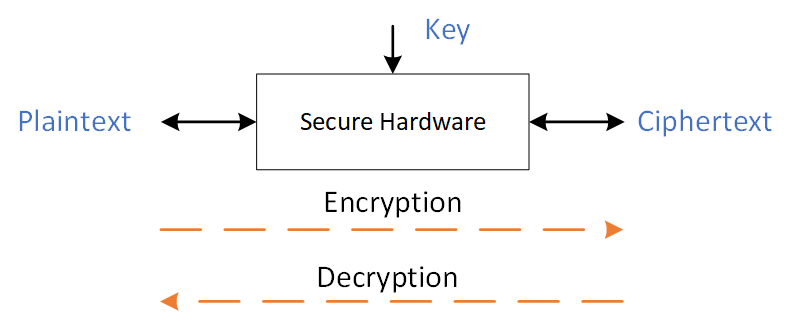
\includegraphics[scale=1.0]{crypto_hw.png}
  \caption{Basic Symmetric Cryptographic Hardware Block Diagram}
  \label{crypto_hw.png}
\end{figure}

\subsection{Rotation}

One of the most common operations in cryptography is called rotation.
Rotation is similar to shifting except anything that is shifted out of
a block gets put back into the block on the other side.  In other
words, a rotation or sometimes called a circular shift is an operation
similar to shift except that the bits that fall off at one end are put
back to the other end.  It is easy to see this as an example.

If we have $n$ that is stored using $8$ bits.
A left rotation of \verb!n = 1110_0101! by $3$ makes
\verb!n = 0010_1111! (Left shifted by 3 and first 3 bits are put back
in least-significant positions.  Fortunately, SystemVerilog (SV) makes
rotation and shifting easy to create with bit-swizzling.

Bit swizzling is SV is achieved with the curly braces \{ and \}.
Using an example from our textbook~\cite{ddca-riscv}, where $y$ is
given as a $9$-bit value
$c_2c_1d_0d_0d_0c_0101$ using bit swizzling operations.  This can be
created in SV by the following statement.
\begin{verbatim}
assign y = {c[2:1], {3{d[0]}}, c[0], 3’b101};
\end{verbatim}
In reality, the \{\} operator is used to concatenate busses. The
\verb!{3{d[0]}}! indicates three copies of \verb!d[0]!.
As stated in our textbook do not confuse the $3$-bit binary constant
\verb!3‘b101! with a bus named $b$.
It is important to note that it is critical to specify the length of
$3$ bits in the constant; otherwise, it would have had an unknown
number of leading zeros that might appear in the middle of $y$.
If $y$ were wider than $9$ bits, zeros would be placed in the most
significant bits.

\section{Data Encryption Standard (DES)}

The Data Encryption Standard (DES) algorithm, adopted by the U.S. 
government in 1977, is a block cipher that transforms $64$-bit data
blocks
under a $56$-bit secret key, by means of permutation and
substitution. It
is officially described in FIPS PUB 46~\cite{fips463}. The DES
algorithm is used for
many applications within the government and in the private sector.

DES uses lots of rotations, swapping or sometimes called
switching, and the use of the exclusive OR operation.
The exclusive OR
or xor 
is useful in that it can be utilized for numbers that have
properties that are sometimes called modular arithmetic.  We will not
go into the theory behind this idea, but you are welcome to explore
more of cryptography in
these great texts~\cite{10.5555/1721909,
  10.5555/2523199}~\footnote{The reference~\cite{10.5555/1721909} is available
electronically in Edmon Low library at
\url{http://library.okstate.edu}.  It an extremely good reference for
those interested in cryptography}.

The symmetric-based cryptographic
algorithm of DES block diagram
can be seen in
Figure~\ref{des-main.png}.  Although Figure~\ref{des-main.png}
looks intimidating, it is just simple combinational logic for each
block.  This will be excellent practice in trying to create some
combinational logic from scratch as well as honing some excellent
debugging skills.  
\begin{figure}
  \centering
  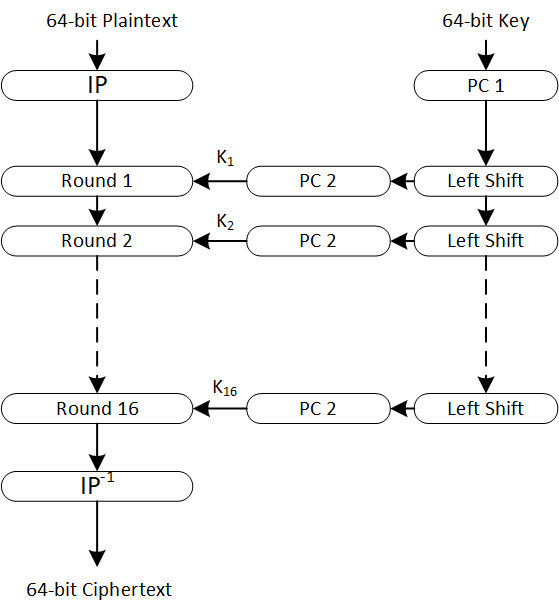
\includegraphics[scale=1.1]{des-main.png}
  \caption{DES Block Diagram}
  \label{des-main.png}
\end{figure}
In order to break down each block, we will break this into two
sections : one for subkey generation (e.g., $K_1$) and the
other for the basic symmetric cryptographic algorithm.

\subsection{SubKey Generation}

In order to start, the best place to start is producing the subkey
generation.  The key generation involves two basic blocks:
\begin{enumerate}
\item Rotation by either $1$ or $2$
\item Two Permutation Choice Box 
\end{enumerate}
The central element to this block is that it produces all sixteen
($16$) subkeys that get used during
encryption and decryption.  More advanced algorithms, for example for
those found in~\cite{10.5555/1721909}, use the same idea with either
the more or less keys to produce more security.

Rotation is performed as explained earlier except that the some blocks are
rotated once and the others block rotates twice.  The only caveat here
is that \textbf{each rotation} should be done by separating each
block of the key
into $28$-bits or broken into two groups.  This kind of confusing as
the key is $64$ bits.  This is because the key has something called
parity bits that protect it from potential errors.

\subsubsection{Parity Bits on the Key}

A parity bit is a bit added to a string of binary code. Parity bits
are a simple form of information to detect any errors.  Parity bits
are generally
applied to the smallest units of a communication protocol, typically
$8$-bits (bytes), although they can also be applied separately to
an entire message string of bits.

The parity bits on the key are done on each group of $8$ bits of the
$56$ bit key making
the total numbers of bits $64$. The locations of the parity bit are
shown in Table~\ref{parity.tbl}.  There are many examples in
engineering for parity but the key is to detect any difference in the
original or transmitted message from the received one.  The parity
within the key is computed simply by XOR'ing of the previous 7 bits.
For example, in Table~\ref{parity.tbl}, $P_7$ is found by XOR'ing the
$7$ $X$ bits and $P_0$ is found by XOR'ing the $7$ $Y$ bits.  This
form of parity is sometimes called odd parity where the occurrences
of bits whose value is $1$ are counted. If that count is even, the parity
bit value is set to $1$, making the total count of occurrences of $1$s in
the whole set (including the parity bit) an odd number.
\begin{table}
  \centering
  {\scriptsize
\begin{tabular}{|c|c|c|c|c|c|c|c|c|c|c|c|c|c|c|c|c|c|c|c|c|c|c|c|} \hline
  $K_{63}$ & $K_{62}$ & $K_{61}$ & $K_{60}$ & $K_{59}$ & $K_{58}$ &
  $K_{57}$ & $K_{56}$ & $\ldots$ &
  $K_{7}$ & $K_{6}$ & $K_{5}$ & $K_{4}$ & $K_{3}$ & $K_{2}$ &
  $K_{1}$ & $K_{0}$ \\ \hline \hline
  X & X & X & X & X & X & X & $P_7$ & $\ldots$ & Y & Y & Y & Y & Y & Y & Y
  & $P_0$ \\ \hline
\end{tabular}
  }
  \caption{Parity Locations within $64$-bit key}
  \label{parity.tbl}
\end{table}

\subsubsection{Rotations within each SubKey}

As indicated previously, the key is rotated or circularly shifted by
$2$.  Rotating is central to the idea in most cryptographic algorithms
as it mixes up the original message similar to how a deck of cards is
rotated.  For the key, rotation happens based on the round that it is
in.  As indicated previously, DES uses $16$ iterations or rounds
and the rotation
happens on different iterations, as indicated in Table~\ref{rotateK.tbl}.
During each iteration, either one or two
circular left shifts on both $C[i-1]$ and 
$D[i-1]$ to get $C[i]$ and $D[i]$, respectively.
\begin{table}
  \centering
  \begin{tabular}{|c|c|c|c|c|c|c|c|c|c|c|c|c|c|c|c|c|c|c|c|c|}\hline
    Iteration \# & 1 & 2 & 3 & 4 & 5 & 6 & 7 &  8 & 9 & 10 & 11 & 12 &
    13 & 14 & 15 & 16 \\ \hline \hline    
    Left Shifts & 1 & 1 & 2 & 2 & 2 & 2 & 2 & 2 & 1 & 2 & 2 & 2 & 2 &
    2 & 2 & 1 \\ \hline
  \end{tabular}
  \caption{Left Rotation within SubKey Generation}
  \label{rotateK.tbl}
\end{table}

Let's try an example to
illustrate this by showing a rotation by two ($2$) on \verb!10_1011_1000!.
To accomplish this rotation, first break the $10$-bits into two groups
of $5$-bits or \verb!1_0101! and \verb!1_1000!.   Then, the rotation
is done on each block separately or:  \verb!1_0110! and \verb!0_0011!
That is, the final rotation will be the concatenation of these two
items or \verb!10_1100_0011!.

\subsubsection{Permuted Choice}

Rotations within cryptographic algorithms are sometimes done with
specific mathematics in mind.  There are several of these ongoing
within DES and they are typically called permutations.  Inside the key
logic, several permutations are computed to generate the
subkey (i.e., $K_i$).  They are called Permutation
Choice~$1$ and Permutation Choice~$2$ or PC-$1$ and PC-$2$ as shown in
Figure~\ref{des-main.png}, respectively.  These
permutations do not use the parity bits discussed earlier as the
parity bits are utilized to detect any errors with the key.
Figure~\ref{des-key.png} illustrates how each of the key bits 
are allocated for each Permuted Choice (PC) function.
The PC-1
operates on $56$ bits of the key where $C_i$ and $D_i$ represent the
left and right side of key logic, respectively.
The PC-1 permutations for the left and right hand side (i.e., $32$
bits for each) are routed as shown in
Table~\ref{pc1.tbl} for each position.   For example, for the left
side of the input, position $0$ output is mapped to position $36$ of
the input key.  
At each round, PC-$2$ takes each
block from PC-$1$ left and right hand side to produce the necessary
subkeys $K_i$ for the encryption and decryption.  The PC-2
permutations for the subkey are shown in
Table~\ref{pc2.tbl}
\begin{table} [b!]
  \centering
\begin{tabular} {|c|c|c|c|c|c|c|c|} \hline
  \multicolumn{7}{|c|}{Left} \\ \hline
  $57$ & $49$ & $41$ & $33$ & $25$ & $17$ & $9$ \\ \hline
  $1$ & $58$ & $50$ & $42$ & $34$ & $26$ & $18$ \\ \hline
  $10$ & $2$ & $59$ & $51$ & $43$ & $35$ & $27$ \\ \hline
  $19$ & $11$ & $3$ & $60$ & $52$ & $44$ & $36$ \\ \hline
  \multicolumn{7}{|c|}{Right} \\ \hline
  $63$ & $55$ & $47$ & $39$ & $31$ & $23$ & $15$ \\ \hline
  $7$ & $62$ & $54$ & $46$ & $38$ & $30$ & $22$ \\ \hline
  $14$ & $6$ & $61$ & $53$ & $45$ & $37$ & $29$ \\ \hline
  $21$ & $13$ & $5$ & $28$ & $20$ & $12$ & $4$ \\ \hline  
\end{tabular}
\caption{Permutation Choice~$1$ (PC-1) Function\protect\footnotemark}
\label{pc1.tbl}
\end{table}
\begin{figure} 
  \centering
  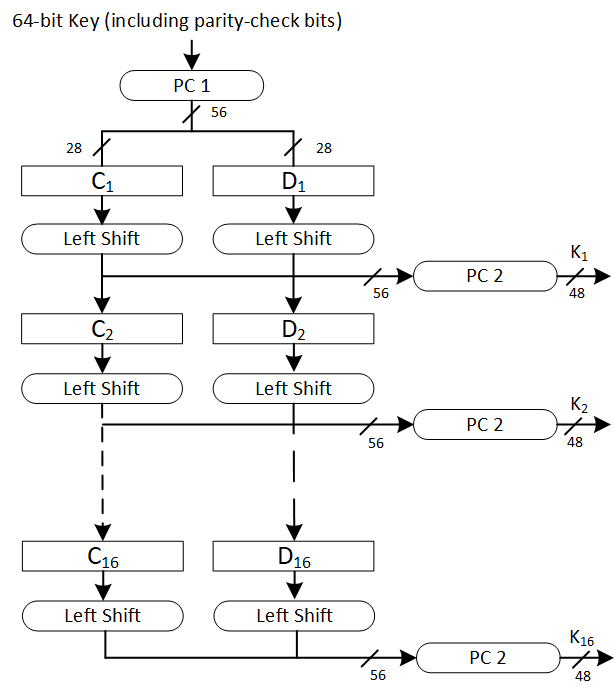
\includegraphics[scale=1.0]{des-key.png}
  \caption{DES SubKey Permutation Diagram}
  \label{des-key.png}
\end{figure}
\begin{table} [b!]
  \centering
\begin{tabular} {|c|c|c|c|c|c|c|c|} \hline
  $14$ & $17$ & $11$ & $24$ & $1$  & $5$  & $3$  & $28$ \\ \hline
  $15$ & $6$  & $21$ & $10$ & $23$ & $19$ & $12$ & $4$ \\ \hline
  $26$ & $8$  & $16$ & $7$  & $27$ & $20$ & $13$ & $2$ \\ \hline
  $41$ & $52$ & $31$ & $37$ & $47$ & $55$ & $30$ & $40$ \\ \hline
  $51$ & $45$ & $33$ & $48$ & $44$ & $49$ & $39$ & $56$ \\ \hline
  $34$ & $53$ & $46$ & $42$ & $50$ & $36$ & $29$ & $32$\\ \hline
\end{tabular}
\caption{Permutation Choice~$2$ (PC-2) Bit Function}
\label{pc2.tbl}
\end{table}

It is important to note that the parity-check bits (namely, bits $4$, $8$,
$16$, $32$, $40$, $48$, $56$, $64$) are not chosen, and they do not
appear in PC-1.  Also, PC-2 selects the $48$-bit subkey for each round
from the $56$-bit key-schedule state from each rotation.  Also, one of
the more difficult elements in electrical and computer engineering
digital applications, in my opinion,
is what constitutes the Least Significant Bit (LSB).  Some programs,
such as MATLAB, have the first entry represented by vector $1$;
however, computers typically represent the first entry by vector $0$.
All of the tables, similar to Table~\ref{pc1.tbl}, will signify the
first entry as $1$ when they really mean bit $0$.  Therefore, please
be wary of this conundrum when implementing the permutations
throughout this laboratory.
\footnotetext{As discussed in
  the text, for this and other permutation tables maps the inputs to the
  outputs (i.e., bits1 through bits64 which should map to position $0$
  to $63$)}.  
  
\subsection{DES Encryption or Decryption Function}

As stated earlier, DES is a symmetric cryptographic algorithm in
that it can be done either way for encryption or decryption.  It is
important to understand the order as shown in
Figure~\ref{des-main.png} making the correct direction is utilized
for encryption or decryption.  Again, this block is another group of simple
combinational logic blocks with it broken down into four basic
blocks:
\begin{enumerate}
\item Initial Permutation (IP)
\item Feistel Block ($f_K$)
\item Switch or Swapping (SW)
\item Inverse Permutation (IP\textsuperscript{-1})
\end{enumerate}

The Initial Permutation (IP) and the Inverse or Final
Permutation (IP\textsuperscript{-1}) blocks are basically moving data
around before each round is processed.  These permutation blocks are
similar to the previous permutation sequences within the subkey
generation, but have different positions for their output.  Both
blocks process $64$ bits of data as inputs and outputs and each
position notation is shown in Table~\ref{ip.tbl} and
Table~\ref{ip2.tbl}. 
\begin{table}
  \centering
  \begin{tabular} {|c|c|c|c|c|c|c|c|} \hline
    $58$ & $50$ & $42$ & $34$ & $26$ & $18$ & $10$ & $2$ \\ \hline
    $60$ & $52$ & $44$ & $36$ & $28$ & $20$ & $12$ & $4$ \\ \hline
    $62$ & $54$ & $46$ & $38$ & $30$ & $22$ & $14$ & $6$ \\ \hline
    $64$ & $56$ & $48$ & $40$ & $32$ & $24$ & $16$ & $8$ \\ \hline
    $57$ & $49$ & $41$ & $33$ & $25$ & $17$ & $9$  & $1$ \\ \hline
    $59$ & $51$ & $43$ & $35$ & $27$ & $19$ & $11$ & $3$ \\ \hline
    $61$ & $53$ & $45$ & $37$ & $29$ & $21$ & $13$ & $5$ \\ \hline
    $63$ & $55$ & $47$ & $39$ & $31$ & $23$ & $15$ & $7$ \\ \hline
\end{tabular}
\caption{Initial Permutation (IP) Function}
\label{ip.tbl}
\end{table}
\begin{table}
  \centering
  \begin{tabular} {|c|c|c|c|c|c|c|c|} \hline
    $40$ & $8$ & $48$ & $16$ & $56$ & $24$ & $64$ & $32$ \\ \hline
    $39$ & $7$ & $47$ & $15$ & $55$ & $23$ & $63$ & $31$ \\ \hline
    $38$ & $6$ & $46$ & $14$ & $54$ & $22$ & $62$ & $30$ \\ \hline
    $37$ & $5$ & $45$ & $13$ & $53$ & $21$ & $61$ & $29$ \\ \hline
    $36$ & $4$ & $44$ & $12$ & $52$ & $20$ & $60$ & $28$ \\ \hline
    $35$ & $3$ & $43$ & $11$ & $51$ & $19$ & $59$ & $27$ \\ \hline
    $34$ & $2$ & $42$ & $10$ & $50$ & $18$ & $58$ & $26$ \\ \hline
    $33$ & $1$ & $41$ & $9$  & $49$ & $17$ & $57$ & $25$ \\ \hline
\end{tabular}
\caption{Inverse or Final Permutation (IP\textsuperscript{-1}) Function}
\label{ip2.tbl}
\end{table}

One of the more challenging elements is when designers and those that
develop these standards refer to specific bits.  Although Electrical
and Computer Engineers are careful with these bits, I find that the
security professionals are sometimes not very specific.  This is
definitely the case for DES as well as other cryptographic algorithms.
If you look at Table~\ref{ip.tbl} and
all the other permutations, they refer to each block starting from the
MSB and move towards the LSB.  Unfortunately, this makes no sense what
bit the standard is referring to and also makes things very confusing.
I have modified the SystemVerilog to
make the permutations easier to follow.  As an example for 
Table~\ref{ip.tbl}, you can see the position is delineated from the
MSB with some minor arithmetic shown in Figure~\ref{ip.sv}.
I left several examples inside the
SystemVerilog files that come with the laboratory to help you follow
along -- please use this
coding to help you make sure you reference the correct bit for any of
the permutation tables that you need to create.
\begin{figure}
\begin{verbatim}
// Initial Permutation
module IP (inp_block, out_block);

   input logic [63:0]  inp_block;
   output logic [63:0] out_block;

   assign out_block[63] = inp_block[64-58];
   assign out_block[62] = inp_block[64-50];
   assign out_block[61] = inp_block[64-42];
   assign out_block[60] = inp_block[64-34];
   assign out_block[59] = inp_block[64-26];
  ...
\end{verbatim}
\caption{Sample SystemVerilog snippet showing position notation for Initial
  Permutation (IP) function}
\label{ip.sv}
\end{figure}


\subsubsection{Round Block}

The main part of this section is called the round block that utilizes
a Feistel function that is
named after the German-American cryptographer Horst Feistel.  Horst
Feistel main work was in developing ciphers for IBM and we call this
block the Feistel block after his pioneering work.

The Feistel block or $f_K$ basically performs the exclusive OR'ing or
XORing on blocks of $32$-bits.  Inside this Feistel block are key
elements of
symmetric cryptographic algorithms called substitution boxes or
sometimes abbreviated as S-box.  S-boxes are utilized in block ciphers to
to obscure the relationship between the key and the ciphertext, thus
ensuring Shannon's property of confusion~\cite{10.5555/1721909}.   For
this lab, I will provide the S-boxes for you so you just have to
compute the round block correctly.  The order of operations in the
round block are as follows:
\begin{enumerate}
\item Split the $64$-bit IP output into two separate blocks of $32$-bits:
  \verb!L[31:0]! and \verb!R[31:0]!.
\item Use the Feistel block to compute a value on the \verb!R[31:0]!
  and $K_i[47:0]$
  that can be used to XOR with \verb!L[31:0]!.  
\item XOR the output of the Feistel block with the \verb!L[31:0]! and
  outputs into the next \verb!R[31:0]! block.
\item The \verb!L[31:0]! output is taken from the previous
  \verb!R[31:0]! effectively swapping the two $32$-bit values.
\end{enumerate}
\begin{figure} [t!]
  \centering
  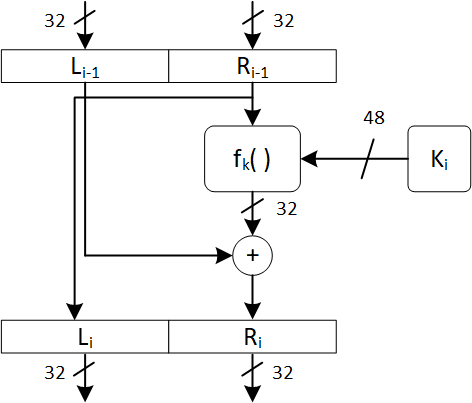
\includegraphics[scale=1.0]{des-round.png}
  \caption{DES Round Block Diagram}
  \label{des-round.png}
\end{figure}
Figure~\ref{des-round.png} shows the basic block diagram of what is
happening during each $16$ rounds.  If you look at
Figure~\ref{des-round.png} closely, you will see that that each left
and right sub-block is swapped during each of the $16$ rounds.

\subsubsection{Feistel Block}

The main Feistel ($f_k$) block utilizes the S-boxes previously
mentioned.  The Feistel block also processes some data before it
enters the S-box as well as when it exits the S-box using an
Expansion Function or Permutation and a Straight D-box Function or
Permutation.

The Expansion
Permutation (EP) follows a predetermined rule. For each
section, input bits $1$, $2$, $3$, and $4$ are copied to output
bits $2$, $3$, $4$, and $5$, respectively. Output bit $1$ comes
from bit $4$ of the previous section; output bit $6$ comes
from bit $1$ of the next section.
Please note that the number of output ports is $48$, but
the input range is only $1$ to $32$.
That is, some of the inputs go to more than one output.
For example, the value of input bit $5$ becomes the value of output
bits $6$ and $8$.  This mapping is shown in Table~\ref{ep.tbl}.  
\begin{table}
  \centering
  \begin{tabular} {|c|c|c|c|c|c|c|c|} \hline
    $32$ & $1$  & $2$  & $3$  & $4$  & $5$ \\ \hline
    $4$  & $5$  & $6$  & $7$  & $8$  & $9$ \\ \hline
    $8$  & $9$  & $10$ & $11$ & $12$ & $13$ \\ \hline
    $12$ & $13$ & $14$ & $15$ & $16$ & $17$ \\ \hline
    $16$ & $17$ & $18$ & $19$ & $20$ & $21$ \\ \hline        
    $20$ & $21$ & $22$ & $23$ & $24$ & $25$ \\ \hline
    $24$ & $25$ & $26$ & $27$ & $28$ & $29$ \\ \hline
    $28$ & $29$ & $30$ & $31$ & $32$ & $1$  \\ \hline        
\end{tabular}
\caption{Expansion Function or Permutation (EP) Function}
\label{ep.tbl}
\end{table}

After the expansion permutation, DES uses the XOR operation on the
expanded right section and the round key. Note that both the right
section and the key are $48$-bits in length. Also note that the round
key or subkey is used only in this operation.  Finally,
the straight Diffusion block
takes in $32$ bits and outputs $32$-bits, as well.  This mapping or
permutation is shown in Table~\ref{dbox.tbl}.  Visually, the Feistel
($f_K$) block is shown in Figure~\ref{des.png}. 
\begin{table}
  \centering
  \begin{tabular} {|c|c|c|c|c|c|c|c|c|c|c|} \hline
    $16$ & $7$  & $20$ & $21$ & $29$ & $12$ & $28$ & $17$ \\ \hline
    $1$  & $15$ & $23$ & $26$ & $5$  & $18$ & $31$ & $10$ \\ \hline
    $2$  & $8$  & $24$ & $14$ & $32$ & $27$ & $3$  & $9$  \\ \hline
    $19$ & $13$ & $30$ & $6$  & $22$ & $11$ & $4$  & $25$ \\ \hline    
\end{tabular}
\caption{Straight Diffusion-box (D-box) Function}
\label{dbox.tbl}
\end{table}
\begin{figure} [t!]
  \centering
  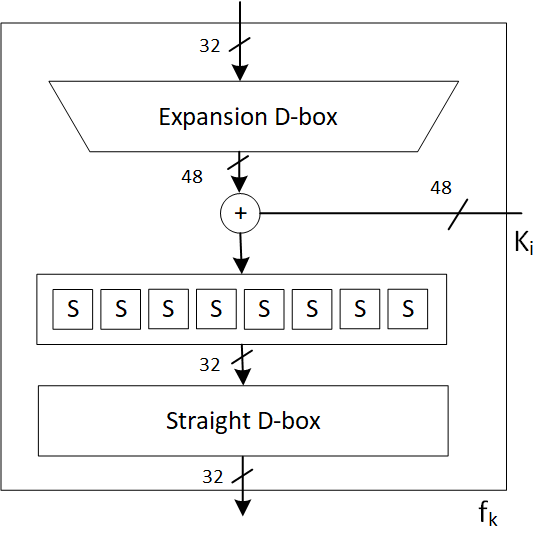
\includegraphics[scale=0.7]{des.png}
  \caption{Feistel ($f_K$) Block Diagram}
  \label{des.png}
\end{figure}

The S-boxes do the real mixing (confusion). DES uses eight ($8$)
S-boxes, each
with a $6$-bit input and
a $4$-bit output.  The $48$-bit data from the second operation is divided
into eight $6$-bit chunks, and each chunk is fed into a box. The result
of each box is a $4$-bit chunk; when these are combined the result is a
$32$-bit text. The substitution in each box follows a pre-determined
rule based on a $4$-row by $16$-column table.  Again, to avoid
confusion this S-box is given to you in SystemVerilog.
Also, as stated previously, the Feistel block operates with each of
the $16$ subkeys (i.e., it is done $16$ times).

\subsection{DES in CBC Mode (DES-CBC)}

For this laboratory, I want you to implement both modes of operation
for the Data Encryption Standard (DES) and have a switch that selects
which version.  These are called Cipher Block Chaining (CBC) and
Electronic Code Book (ECB).  The DES CBC encryption process requires a
$64$-bit cryptographic
key similar to the ECB mode which is the default mode.  There are
other modes, but we will only implement CBC and ECB for this laboratory.
The DES CBC encryption process also requires a $64$-bit Initialization
Vector (IV).

The process in implementing CBC is similar to ECB except that it
requires an IV input, as well.
The first step to initiating a CBC is to XOR the first
of many plaintext blocks with an IV -- a unique, fixed-length
conversion function -- to create a random, or pseudorandom, output.
That is, it is simply that the plaintext is XOR'ed with the
Iniatialization Vector (IV) right in the beginning of the process.
\begin{eqnarray*}
  Plaintext_{new} & = & IV \oplus Plaintext_{input}
\end{eqnarray*}

The key to this is that the IV must be processed in the beginning
during encryption and towards the end in decryption.  You can see get
the idea visually in Figure~\ref{overview-block.png}.
\begin{figure} [t!]
  \centering
  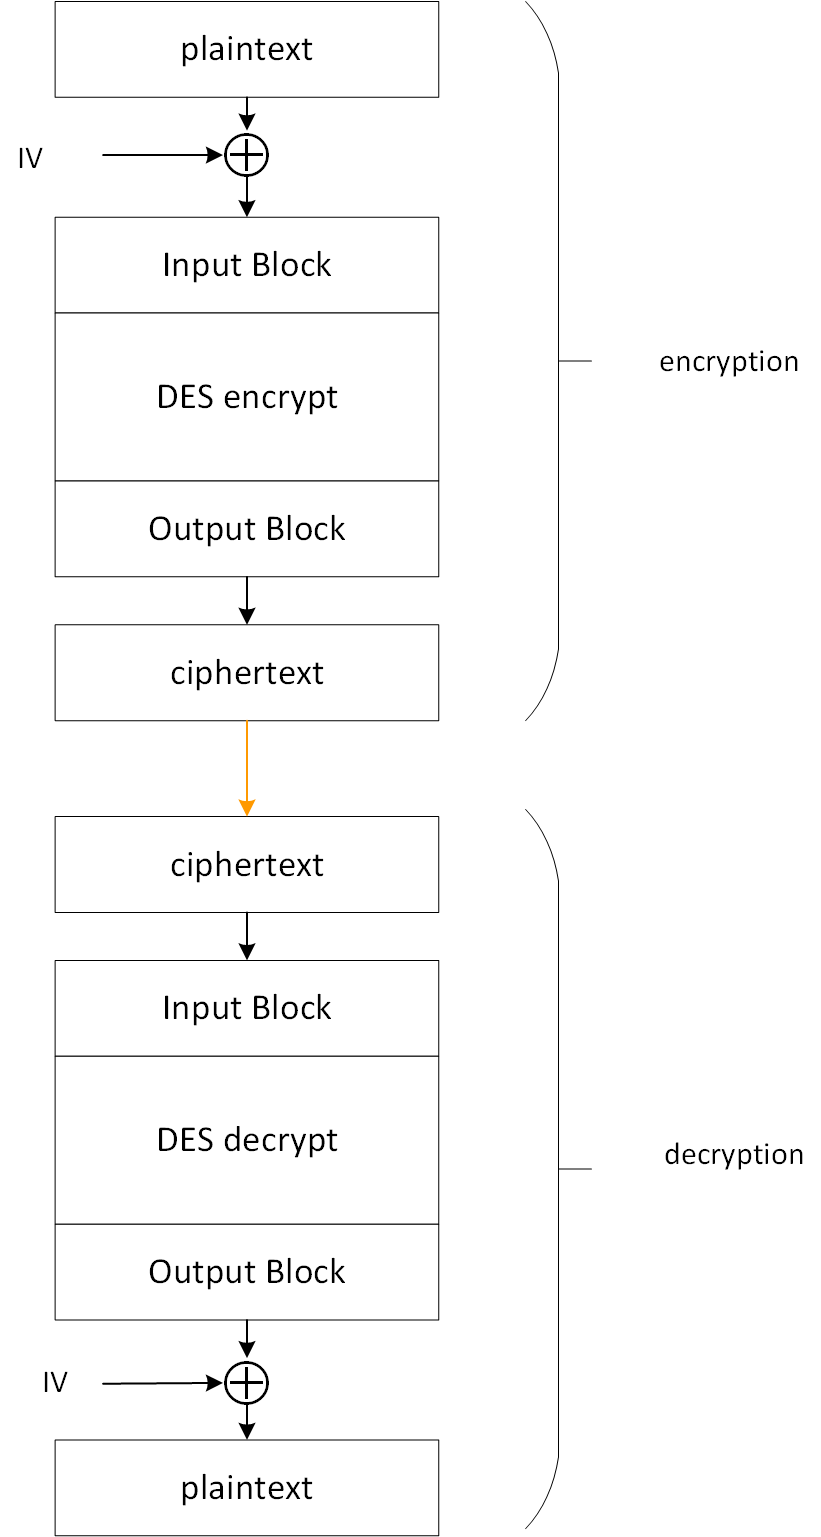
\includegraphics[scale=0.5]{overall-block.png}
  \caption{Encryption/Decrypption Overall Block Diagram}
  \label{overview-block.png}
\end{figure}


\subsection{Encryption or Decryption}

Encryption or decryption can be produced from the same block as shown in
Figure~\ref{des-main.png}.  This is where the name symmetrical
cryptographical algorithm comes from.  The only difference is the
order of operations and what Key is being
used (i.e., $K_1$ or $K_2$).
That is, decryption uses the same algorithm as encryption, except that
the subkeys $K_1 K_2, \ldots, K_{16}$ are applied in reversed order.
Your design should have an input that tells it whether to
encrypt or decrypt your block.

\subsection{Summary of Algorithm}

To give a summary of the algorithm, we will show the pseudo-code of
what is happening.  Pseudo-coding is done to give a very high-level
view of an algorithm.  As stated previously, the algorithm is not
difficult, it just has many steps.  If you know what has to happen at
each step, it become easy to implement, especially with SystemVerilog.
Algorithms~\ref{alg:key},~\ref{alg:encrypt},~\ref{alg:decrypt} show
the pseudo-code for each.  
\begin{algorithm}
\caption{SubKey Schedule}\label{alg:key}
\begin{algorithmic}
\Require $key$
\Ensure \verb!key[63:0]! with odd parity
\State $\{C[0], D[0]\} = PC1(key)$
\For{$1 \leq i \leq 16$}
\State $C[i] = LS[i](C[i-1])$
\State $D[i] = LS[i](D[i-1])$
\State $K[i] = PC2(\{C[i], D[i]\})$
\EndFor
\end{algorithmic}
\end{algorithm}

\begin{algorithm}
\caption{Encipherment}\label{alg:encrypt}
\begin{algorithmic}
\Require plain block, \verb!K[1]! through \verb!K[16]!
\State $\{L[0], R[0]\} = IP(\text{plain block})$
\For{$1 \leq i \leq 16$}
\State $L[i] = R[i-1]$
\State $R[i] = L[i-1] \oplus f_k(\{R[i-1], K[i]\})$
\EndFor
\State $\text{cipher block} = FP(\{R[16], L[16]\})$
\end{algorithmic}
\end{algorithm}

\begin{algorithm}
\caption{Decipherment}\label{alg:decrypt}
\begin{algorithmic}
\Require cipher block, \verb!K[1]! through \verb!K[16]!
\State $\{R[16], L[16]\} = IP(\text{cipher block})$
\For{$1 \leq i \leq 16$}
\State $R[i-i] = L[i-1]$
\State $L[i] = R[i-1] \oplus f_k(\{L[i-1], K[i]\})$
\EndFor
\State $\text{plain block} = FP(\{L[0], R[0]\})$
\end{algorithmic}
\end{algorithm}

\subsection{Power, Performance and Area (PPA)}

For this laboratory, we are going to analyze the design with better
PPA.  That is, you should analyze your design for Power, Performance
and Area.  As opposed to previous laboratories, this procedure that
will be documented here is more robust and gives better numbers that
you can use to assess whether your design is credible or not.  As with
any digital design, engineers use PPA to assess the level of
difficulty, challenge, and effort needed for a design.

To assess your PPA for this design, you should determine its PPA after
implementation.  This is because some of the PPA results (e.g.,
timing) are not adjusted properly until the Implementation phase.  The
Implementation phase typically places and routes the design onto the
FPGA by connecting all the logic blocks that we read about in the
article that we looked at in Lab 0~\cite{7086413}.

To obtain the PPA results, you first have to run through your design
making sure that it is implemented correctly.  Then, you need to add
the following reports after the route stage (i.e., during
Implementation):
\begin{enumerate}
\item \verb!report_utilization! : Area
\item \verb!report_timing! : Performance
\item \verb!report_power! : Power
\end{enumerate}
You can the reports you need by clicking on the reports tab, right
mouse clicking, and then adding the report you need, as shown in
Figure~\ref{reports1.png}.  Once you add the report, it is easiest to
re-run the implementation to get the report.  Clicking on the option
gets you specific report which you can save.
\begin{figure} [b!]
  \centering
  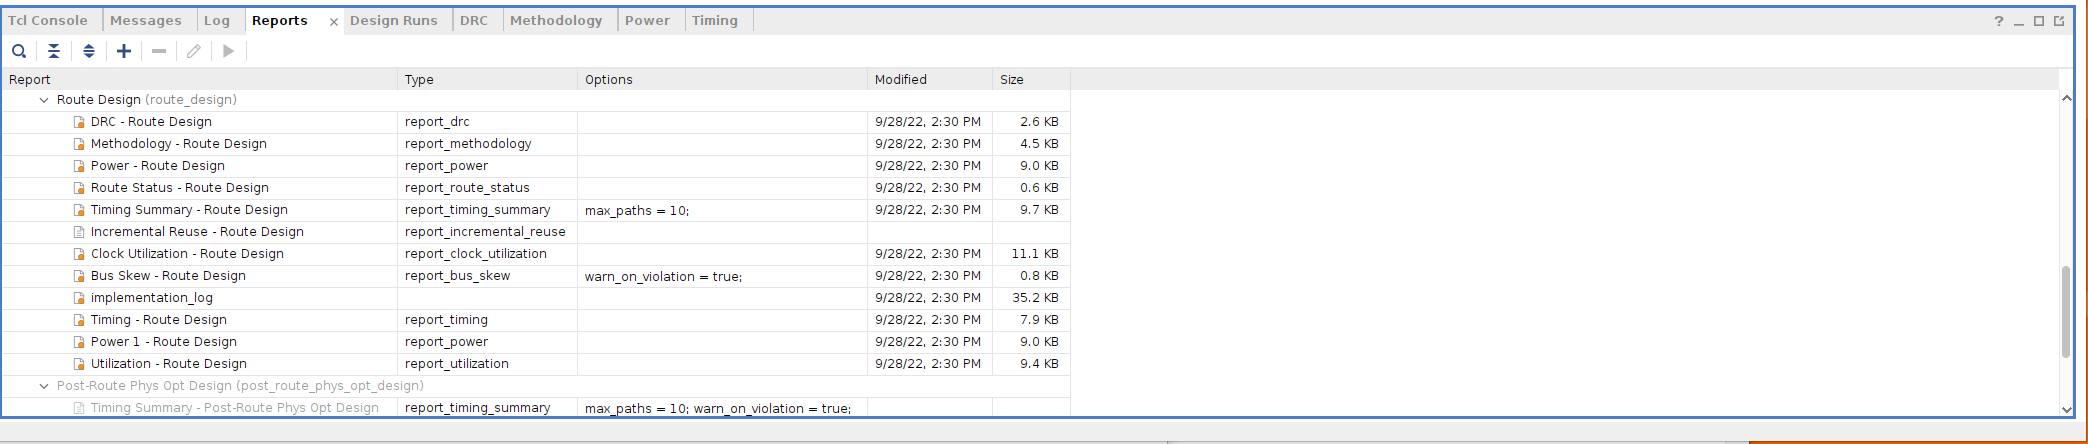
\includegraphics[scale=0.3, width=\columnwidth]{analysis.png}
  \caption{Reports Window within Xilinx Vivado}
  \label{reports1.png}
\end{figure}

  
\section{Tasks}

Most of the blocks and their operation
have been given to you to help you understand the
problem better.
For those that are interested in more about cryptography and how
hardware can impact the future, I encourage you to read more about it
through searching on the Internet as well as this great
reference~\cite{10.5555/1721909}.
One of the hard parts of any engineering problem is
to understand what is going on and making sure you are correct.
Therefore, digital designers rely heavily on getting good data to make
sure they are right.  Typically, this is done either on paper and
pencil or through software.

We will use software for this approach
and use a piece of software written in Java.
If you need
to install Java on your machine at home or laptop, go to
\url{https://www.oracle.com/java/technologies/downloads/#java16} and
download the appropriate version.
The main part of the encryption output looks like the following in
Figure~\ref{des.java} after
typing \verb!java DES!.  The plaintext and
key are inside the \verb!DES.java! program
and can be easily modified, however, I wrote a method in Java that
checks the
parity so make sure you have a good key.  For example, in round 1,
\verb!L_1 = 0x8C13_B66C!, \verb!R_1 = 0xF3EF_C169! and
\verb!K_1 = 0x2080_66A2_53BA!.  As seen by the output in
Figure~\ref{des.java}, the plaintext \verb!0x2579_DB86_6C0F_528C! with
a key of \verb!433E_4529_462A_4A62! produces the correct ciphertext of
\verb!ECB5_4739_A183_2EC5!.
This could be checked by taking the ciphertext and decrypting it
through the algorithm.  Since the algorithm is symmetric, it utilizes
the same procedure for encryption or decryption except that the keys
are reversed.
There are several DES calculators
available online through Google search if you wish to validate the
result this way, as well. 
\begin{figure}
\begin{verbatim}
Original plain Text:    2579DB866C0F528C
Key:                    433E4529462A4A62
IV (for CBC mode):      0000000000000000

Encryption:

After initial permutation: 5646B9278C13B66C
After splitting: L0=5646B927 R0=8C13B66C

Round 1	        8C13B66C F3EFC169 208066A253BA
Round 2	        F3EFC169 25DAF255 C0B6508F6DC2
Round 3	        25DAF255 1890CFBF 44D6422CC355
Round 4	        1890CFBF AFB98FA0 62D142D3C4C6
Round 5	        AFB98FA0 8F76DBD7 28C143CC8789
Round 6	        8F76DBD7 C176D0E5 21411B9A764D
Round 7	        C176D0E5 C7401A8C 2501917AD3A0
Round 8	        C7401A8C B748825A 170891906D2B
Round 9	        B748825A 61239171 084949255DD5
Round 10        61239171 FE28B577 01690D8B80F3
Round 11        FE28B577 CDB650DE 012D81C7CF05
Round 12        CDB650DE 8B8270E5 512CA11A07DC
Round 13        8B8270E5 DDDBEE19 D1A480D9D185
Round 14        DDDBEE19 5F82D63F 5086864266A9
Round 15        5F82D63F B35B4964 709006FA390D
Round 16        B35B4964 850AC7BE C03E202F8437

Cipher Text: ECB54739A1832EC5
\end{verbatim}
\caption{Java output for encryption from DES.java}
\label{des.java}
\end{figure}

Verification is extremely difficult
because there are so many moving parts.  Use the
Java program to verify each block out of the HDL.  Although the Java
works based on bytecodes that are interpreted, I have found that some
machines have problems reading the Java bytecodes.  I am still not
quite sure why this is the case, however, there is an easy fix.
Therefore, I included a
Makefile that I wrote that allows you to compile the Java correctly.
Please type the following if you are having problems running the
code.  To run the tool, type \verb!java DES! at the command prompt.
\begin{verbatim}
make clean
make
\end{verbatim}
If you cannot run \verb!make! on your Windows box, just type the
\verb!javac! commands found within the Makefile on each Java file
(i.e., \verb!javac -d . -classpath . DES.java!).  

The main tasks for this laboratory
will be the following elements:
\begin{enumerate}
  \item Design the DES combinatianal block for both encryption and
    decryption in SystemVerilog and simulate with ModelSim.
  \item Use the Java verification tool to help you with verifying the
    correct operation within ModelSim.  There is also a decent online
    DES calculator available at \url{https://emvlab.org/descalc/} that
    shows a simplified input/output value from either encryption or decryption.  
  \item Implement a switch that indicates ECB or CBC modes and
    processes everything accordingly.
  \item Test at least $10$ random messages (i.e., plaintext) using
    $2$ random keys for both encryption and decryption.
  \item After verifying your design with a testbench in ModelSim,
    implement your design on the DSDB board and use the    
    $7$-segment display to display your plaintext and ciphertext.
    Since you only have four $7$-segment displays, you will not be
    able to show the entire plaintext, ciphertext or key, so you will
    have to figure a way to verify the operation.
  \item You should also design an option that displays a LED if the
      key is correct (i.e., that parity is correct or that it is
      odd).  Your hardware should work regardless of parity because it
      does not use these bits when computing the subkeys, but a LED
      should be lit up if the key is bad - i.e., it does not have odd
      parity.  The java code comes with a method to help check whether
      the parity is odd to help you validate the parity.
  \item Use the push buttons, switches, and LEDs to help you input
    your plaintext as well as debug operation and prove that your
    design works on your DSDB board.
    \item You should also analzye the PPA impact on your design. 
\end{enumerate}
This laboratory should involve \textbf{only combinational logic} and be
straight forward in creating Boolean logic with SystemVerilog.
Again, there are many parts to this design and based on experience, I
believe it will be easier to debug the key generation first and then
once this works, debug the encryption/decryption next.  The key
generation is slightly easier than operations like the Feistel block,
so it will optimize your design process if you focus on this block
first.  However, I would use the strategy that works the best for you.

\subsection{Testing and Stubbing Code}

You should use the testbenches you utilized for Lab0 and Lab1 to help
you test your design.  The design is completely combinational and
should not be any different in terms of structure than both of these
labs.  To get full credit, you should demonstrate that your design
works for both encryption and decryption by testing at least $10$
plaintext messages using at least $2$ different keys.  This is
basically testing $20$ vectors - the more vectors tested and the
methodology you use could possibly
earn you extra credit on this laboratory.

I have also given you some freebies to help you with this lab.  When
writing HDL or software, it is sometimes useful to \textit{stub} your
code.  A stubbed piece of code is a blank piece of software that has
most of your functions you believe will work for your design.
Fortunately, I have stubbed out your SV for you and you can use this
as a guide.  I also put some comments in the SV to help you know where
to instantiate certain items.
Inside the SV, I have also included the complete S-boxes
which are the substitution boxes you will use for
this laboratory.  All of the S-boxes work by giving them $6$-bits and
they produce $4$-bits as an output, as indicated previously.

I have also utilized a more advanced testbench that reads your
key, plaintext, and ciphertext from a file.  These are included in the
\verb!des.tv! files and $4$ examples are given.  The testbench should
read in the values on each edge of the clock as in Lab 1.  Although
this testbench outputs data to a file, you will find more information
can be found through debugging in ModelSim as documented in the next
subsection.

\subsection{Getting to know ModelSim and Debugging more in depth}

ModelSim is a professional Hardware Descriptive Language tool for
simulation and verification.  It has many neat features to help you
with debugging.  Although testbenches are the main vehicle for
understanding how to test a digital system, using ModelSim can save
you hours and days in debugging a design.  Therefore, we are also
going to introduce some new features of ModelSim that you should use
to help you with this laboratory. I also encourage you to use the
testbench skills you learned from Lab 1.

The features you will use in ModelSim are the \textit{Sim} and
\textit{Objects} window.  Normally both of these windows are present
when running a DO file, however, sometimes I find that they do not
open properly.  You may need to activate them in the View menu at the
top of ModelSim.  They should look like Figure~\ref{modelsim.png} when
activated.  Both of these windows are utilized with the Wave window.
\begin{figure} [t!]
  \centering
  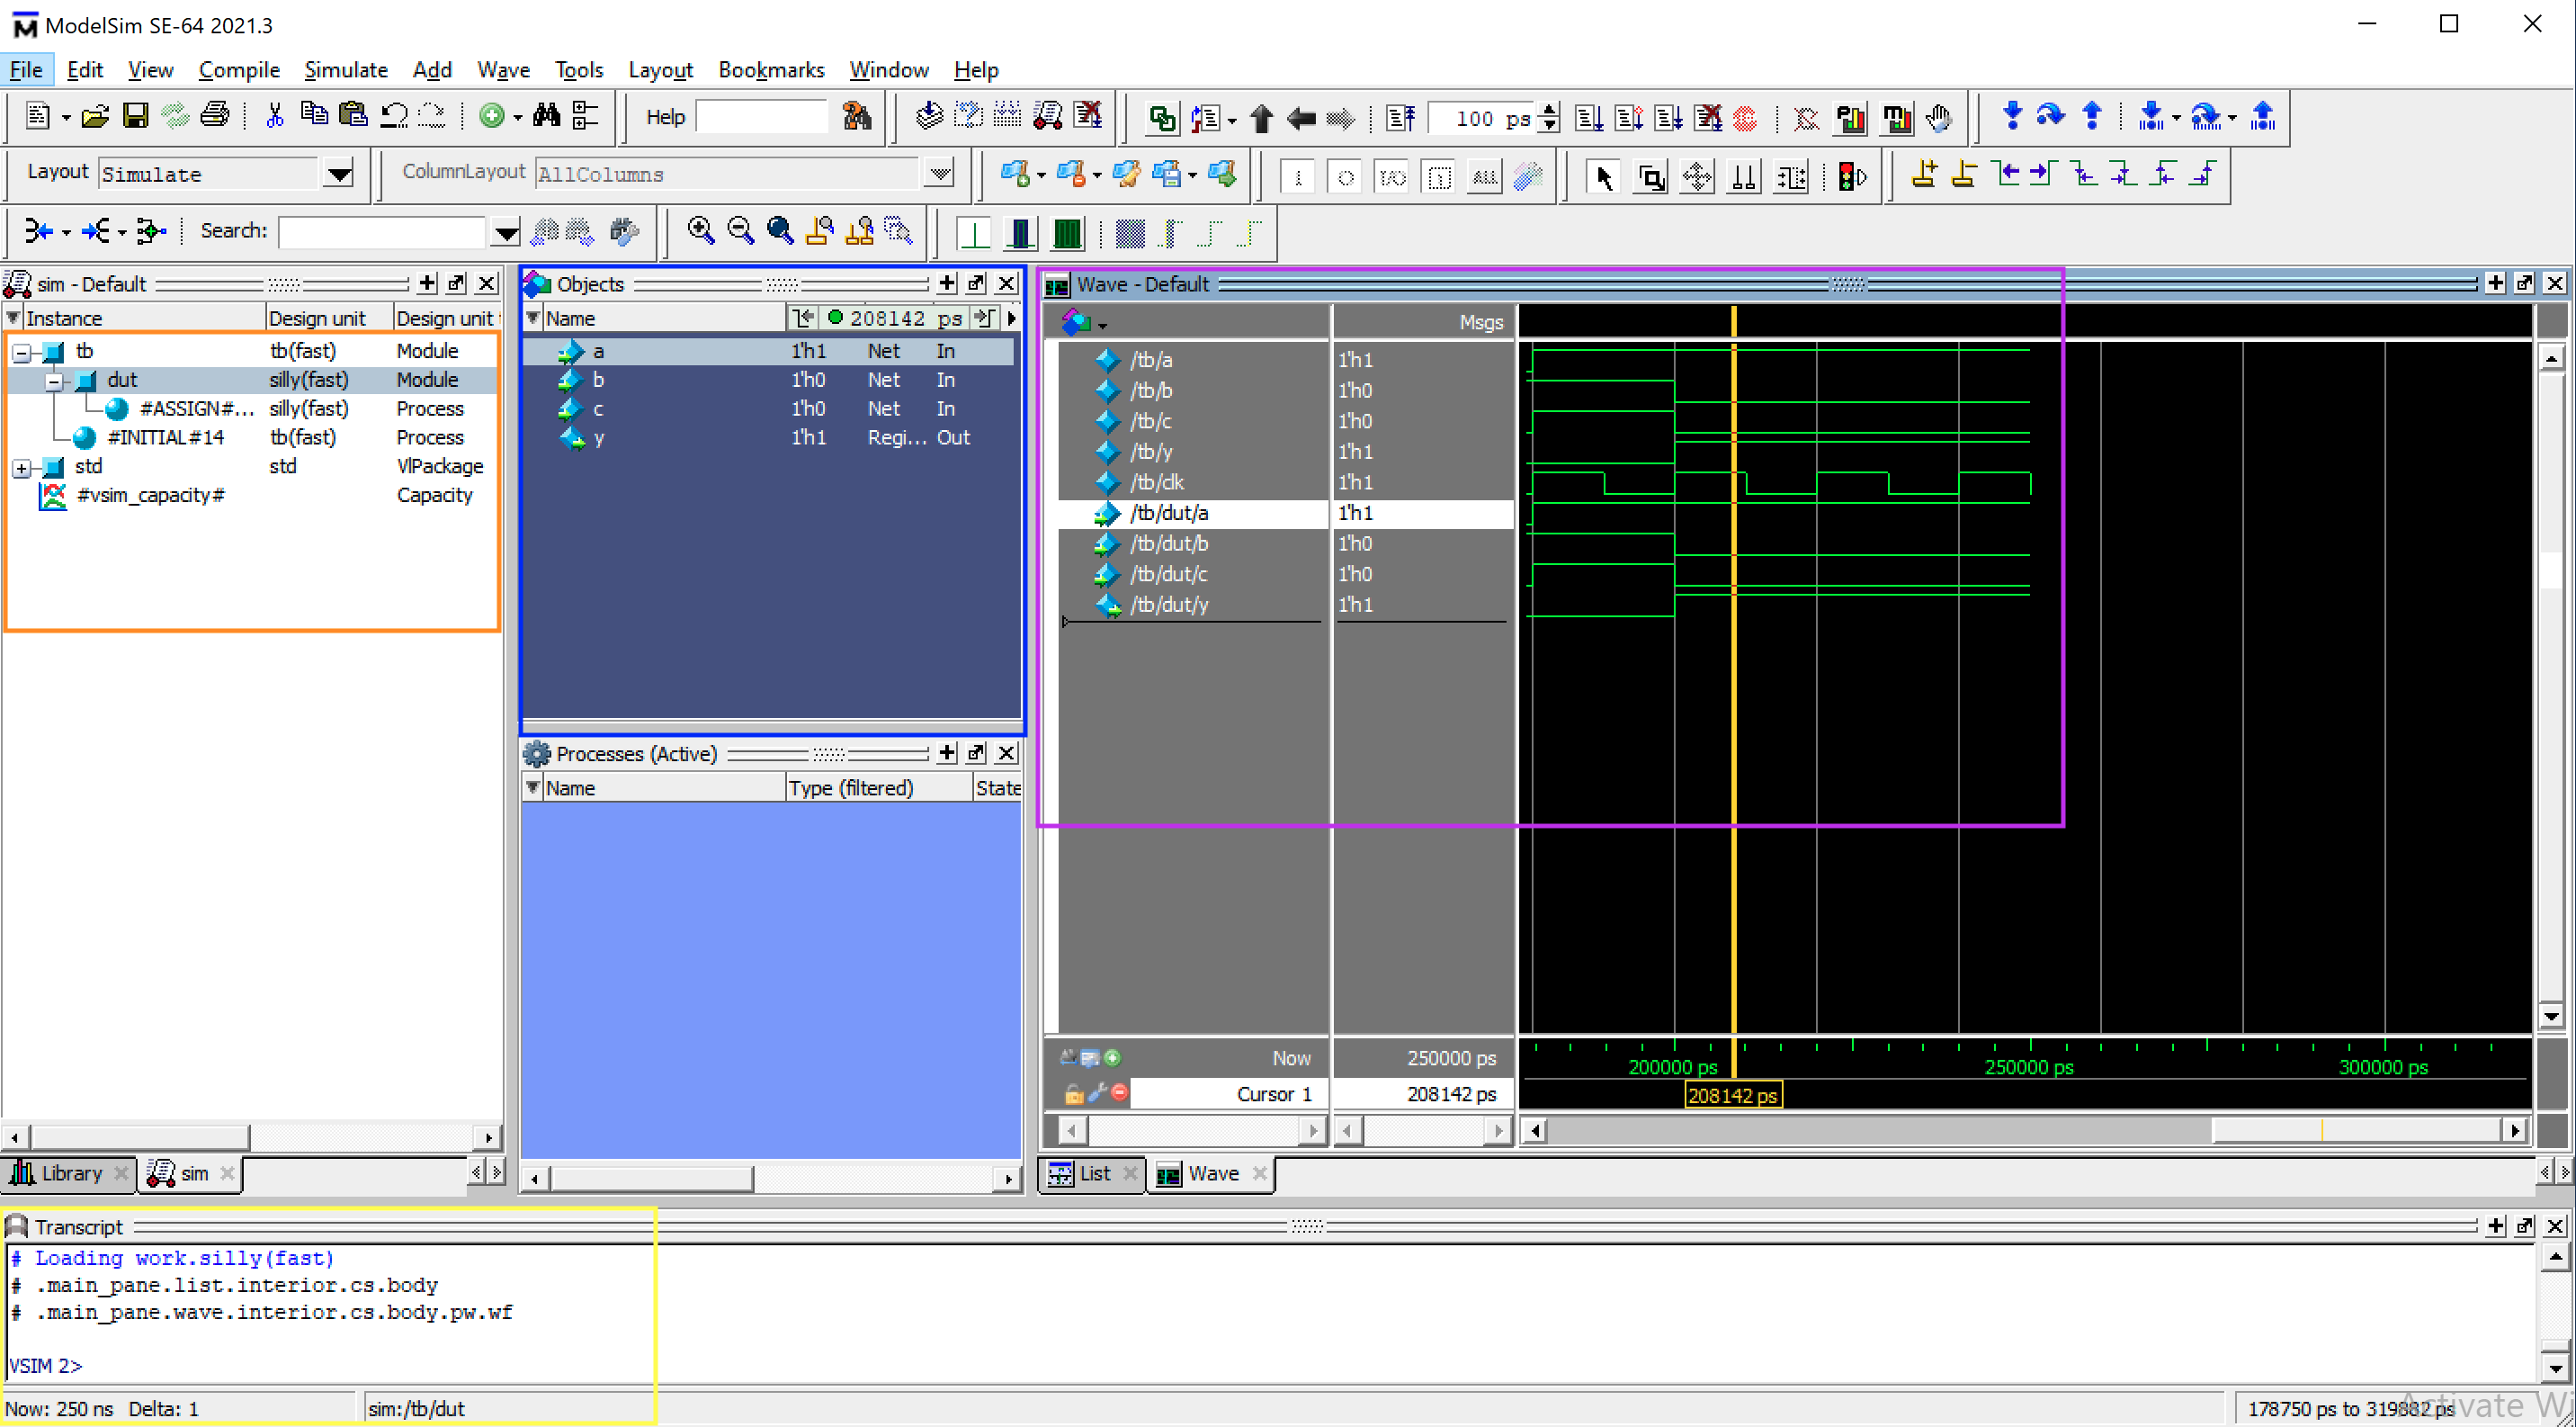
\includegraphics[scale=0.3]{modelsim.png}
  \caption{ModelSim Sim and Objects Window}
  \label{modelsim.png}
\end{figure}

To use the two windows effectively, you should use the \textit{Wave}
to see the data at a certain time.  First, move your cursor to the
time you wish to investigate something - you should see a yellow line
indicating the time you are observing the data.  Next, you
should navigate to the
hierarchy of the module you wish to verify in the \textit{Sim} window
and the \textit{Objects} window will display all signals and values
that for that instance at a given time.  You might need to play around
with using these two windows together with the \textit{Wave} window,
but once you do you will find that its easy to debug what each block
is producing at a given time.

The "sim" window (orange) contains the hierarchy of the design.  The
top level shows the test bench (tb) with a expandable button to the
left.
By clicking the "+" it opens the hierarchy for all modules
instantiated in tb.  Clicking on the name of the instance changes
which objects (blue) are visible in the "objects" window.  You can
also add an
object to the wave by right clicking on the name of the object in the
"objects" window "Add Wave".  Your testbench and modules may use
different names but the same process applies to add signals to the
wave (purple).

You can save the wave by clicking in the wave window then clicking the
brown colored floppy disk icon in the toolbar.  (Third icon from the
left)  The saved file only contains the configuration of the wave not
the actual data. This allows you to recall the wave if you restart
modelsim at a later time.  To recall the wave you can type "do <name
of wave file> in the transcript (yellow).  You can also add this to
the do file so it always pulls up your wave every time the simulation
is run.

Modelsim has many extra features which can greatly aid in your debugging.
First let's discuss some tips and tricks.
\begin{itemize}
\item  If the toolbar gets disorderly, right click in the toolbar and
  select reset.
\item Signals in the wave by default show the full path name.  This can
  be changed to just the lowest level of hierarchy by clicking the
  ``toggle leafs name'' button in the lower left of the wave shown in
  Figure~\ref{modelsim-tips1.png}  
\item Zoom buttons are confusing.  The ``+'' zoom in is mostly useless.
  Use the yellow upside down ``T'' with magnifying glass to zoom in
  at the cursor, as shown in Figure~\ref{modelsim-tips2.png} in red.
\item The ``-'' zoom button works as expected.
\item If you select a signal in the wave viewer, ``Tab'' and ``Shift + Tab''
  will move the cursor to the next transition.
\item A multibit bus can be search for a specific value using the ``Search''
  buttons in the toolbar.  The blue left and right allows to the right of
  the ``Search'' button will search backwards (left) or forwards (right)
  in time, as shown in Figure~\ref{modelsim-tips2.png} in green.
\end{itemize}

At the risk of complicating things the ``data flow'' window can be very
helpful when debugging red X's.  Either in the objects window or the wave
window right click a signal and select ``Add to dataflow''. This opens
a new window where you can right click and select ``ChaseX'' or ``TraceX''.
These allow you to quickly find the source of an X.  If this does not make
sense you can skip.
\begin{figure} [t!]
  \centering
  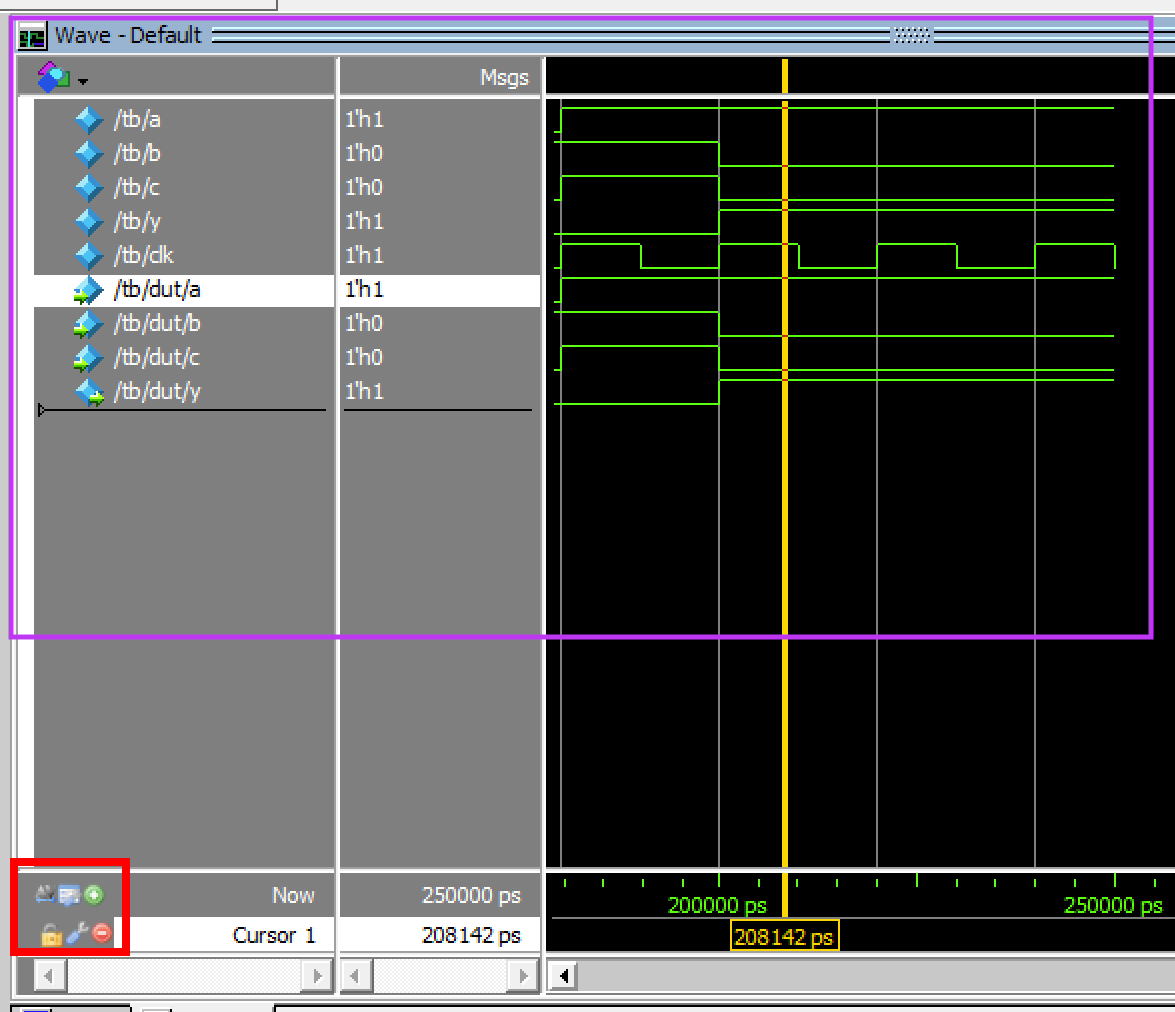
\includegraphics[scale=0.4]{modelsim-tips1.png}
  \caption{ModelSim toggle leafs. In the red box, the left-most box is the ``Now'' row.}
  \label{modelsim-tips1.png}
\end{figure}
\begin{figure} [t!]
  \centering
  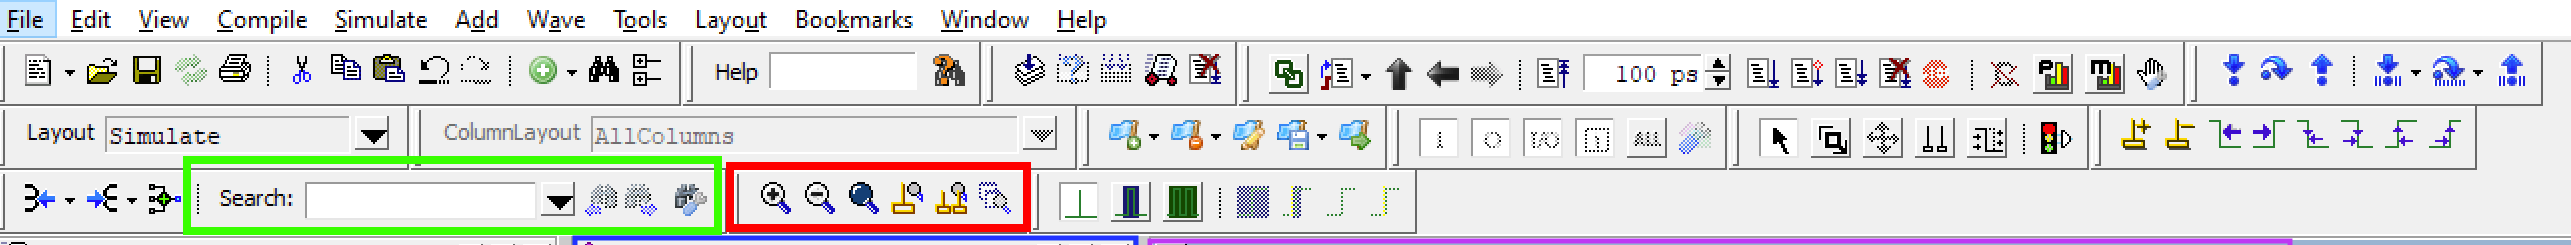
\includegraphics[scale=0.32]{modelsim-tips2.png}
  \caption{Search inside the green box and zoom controls in the red box.}
  \label{modelsim-tips2.png}
\end{figure}

\subsection{Extra Credit}

If you get done early, you can attempt some extra credit.  However, I
would only try this option if you get everything verified within your
design.  
One possible improvement is to work on optimizing the verification
of your design.  You can do any other modification (e.g., re-writing
the Java code) or the DES implementation in Java, as well.
%Yet another piece of extra credit is analyzing how fast you can run
%DES through the FPGA.  This will involve using Vivado to analyze how fast your
%design can be and doing some calculations on how fast you can encrypt
%and decrypt your data.

You also have the opportunity to enhance the DES and creating 3DES
which is sometimes called triple DES.  Triple DES is still used in
some application and even used for some Microsoft keys that were used
when purchasing software; however, I think they stopped using these
several years ago.  Interestingly, four out of
$2^{56}$ possible keys are called weak keys.
A weak key is the one that, after parity removal operation,
consists either of all $0$s, all $1$s, or half $0$s and half $1$s.
These keys are shown in Table~\ref{weak.tbl} and I encourage you to
try these keys in your hardware but do not use them in real life ;).
\begin{table}
  \centering
  \begin{tabular}{|c|c|c|c|c|}\hline
    Keys with parity ($64$ bits) & Actual key ($56$ bits)
    \\ \hline \hline
    \verb!0x0101_0101_0101_0101! & \verb!0x00_0000_0000_0000! \\ \hline
    \verb!0x1F1F_1F1F_0E0E_0E0E! & \verb!0x00_0000_0FFF_FFFF! \\ \hline
    \verb!0xE0E0_E0E0_F1F1_F1F1! & \verb!0xFF_FFFF_F000_0000! \\ \hline
    \verb!0xFEFE_FEFE_FEFE_FEFE! & \verb!0xFF_FFFF_FFFF_FFFF! \\ \hline
  \end{tabular}
  \caption{DES Weak Keys}
  \label{weak.tbl}
  \end{table}


\section{Submission}

You should electronically hand in your HDL (all files that you want
us to see) into Canvas.
You should also take a printout of your waveform 
from your ModelSim simulation.  
Only one of your team members should upload
the files and/or lab report. Please contact
James Stine
(james.stine@okstate.edu) 
for more help.  Your
code should be
readable and well-documented. In addition, please turn in additional
test cases or any other added item that you used. 
Please also remember to document everything in your Lab Report using
the information found in the Grading Rubric.


    
\bibliographystyle{IEEEbib}
\bibliography{lab2}

\end{document}
